\subsection{Using Damaris for In Situ Visualization}\label{sec:insitu_eval}

In this section, we evaluate how Damaris can be used for in situ visualization by
studying two aspects of our framework. First we show the adaptability
and ease of use of Damaris by quantifying required code modifications for data accesses
in existing simulations. 
We then evaluate the performance benefits of using 
dedicated cores in terms of scalability of the visualization process,
and impact on simulation performance.

\subsubsection{Impact on Code Instrumentation and Adaptability}

We compared our framework with two representative software packages 
used for tightly-coupled ISV, VisIt and ParaView, 
in terms of code modification and adaptability. 
We conducted this study around the particular 
scenario of a rectilinear mesh with temperature values. This scenario, 
corresponds to the sample code presented in Section~\ref{sec:damaris_viz:DamarisInSitu}.
It will also be applied in  Section~\ref{sec:damaris_viz:Experiments} to the CM1 
simulation, and is characteristic of a climate simulation handling a 3D 
\emph{temperature} array of double precision values mapped onto a rectilinear grid.
%Listing~\ref{lst:basesim} introduces the corresponding portion of the simulation
%code where these arrays are allocated.

%\begin{Listing}[t]
%	\lstinputlisting[language=C]{listings/base_sim.c}
%	\caption{Data allocation in the original simulation.}\label{lst:basesim}
%\end{Listing}

%Section~\ref{sec:DamarisInSitu:visit} presented how this scenario is handled
%by our framework through a six-lines code instrumentation and a short XML 
%description. In the following we compare this instrumentation to two widely used
%software: VisIt and ParaView.

\paragraph{Damaris vs. VisIt}
VisIt is one of the major software for
parallel scientific visualization. It offers in situ visualization capabilities through the 
\emph{libsim}~\cite{whitlock2011parallel} library. This library allows the simulation 
to act as a parallel rendering engine when receiving commands from a VisIt client.
Visualization tasks can also be scripted to run 
without user intervention. VisIt works directly on the data provided by 
the simulation without making a copy. 
%This leads to a major reduction of memory requirements. 
The ``Getting data into VisIt'' manual~\cite{gettingdataintovisit}
provides a complete documentation on how to instrument a simulation. This 
instrumentation requires to restructure the simulation's main loop in order to 
periodically check for pending visualization requests from the user, using the 
\texttt{VisItDetectInput(...)} function. When a connection is started with a 
client, the simulation has to provide callback functions to the \emph{libsim} 
library. These callbacks access data, metadata and issue commands. 
In our example, two callback functions are provided in addition to the callback 
functions required for metadata access and response to commands. 
Listing~\ref{lst:visitaccess} presents an overview of these data access functions.

%%%%%%%%%%%%%%%%%%%%%%%%%%%
\begin{Listing}[t]
	\lstinputlisting[language=C]{listings/visit_access.c}
	\caption[In situ data access functions using VisIt]{Data access functions 
	for our sample application using VisIt. The 
	first function retrieves the mesh coordinates, while the second retrieves 
	the temperature field. The two last lines register the two functions as 
	callbacks handling data accesses. This sample code does not show the 
	modifications to the simulation's main loop.}
	\label{lst:visitaccess}
\end{Listing}

In contrast, the code modifications required by Damaris boil down to the few
lines presented in Listing~\ref{lst:damarisaccess} in Section~\ref{sec:damaris_viz:DamarisInSitu}.

In addition to our previous example and to quantify more precisely the modification costs
in VisIt and in Damaris, we rewrote the examples provided in 
VisIt's source to work with Damaris. Table~\ref{tab:instrumentation:visit}
summarizes the number of lines of code required to instrument these examples 
with the two frameworks.\footnote{These numbers might differ our previous work~\cite{dorier2013damarisviz}, 
as a newer version of Damaris with a slightly different API was used here.} 
We removed all comments and blank lines in order to
count only the lines of code relevant to the simulation/visualization coupling. 
Note that all of these examples except the 
last are serial. The last one, \emph{life.c}, requires further 
modifications with VisIt to provide callback functions for collective communications.
All these codes (including the unmodified ones from VisIt) are available in the 
Damaris release.\footnote{See \url{http://damaris.gforge.inria.fr}.}

\begin{SCtable}
%\center
 \caption[Amount of code modifications in example codes using VisIt and Damaris]{Code 
   modifications of different VisIt examples. Damaris requires
   code modifications and an external XML file.}\label{tab:instrumentation:visit}
   \begin{tabular}{|l|c|c|c|}
      \hline
   & \textbf{VisIt} & \multicolumn{2}{c|}{\textbf{Damaris}} \\
      \hline
Simulation   & C  & C & XML \\
      \hline
      curve.c  & 144 lines & 8  lines & 32 lines\\
      mesh.c   & 167 lines & 10 lines & 46 lines\\
      var.c    & 271 lines & 15 lines & 63 lines\\
	  point.c  & 161 lines & 9  lines & 33 lines\\
	  blocks.c & 188 lines & 10 lines & 45 lines\\
      life.c   & 305 lines & 10 lines & 40 lines\\
      \hline
   \end{tabular}
   
\end{SCtable}

These number of lines clearly show that Damaris greatly simplifies the code
modifications required to couple existing simulations with visualization tools,
thus helping users adopt in situ visualization as an alternative to offline
visualization.

\paragraph{Damaris vs. ParaView}
Like VisIt, ParaView is based on VTK. 
The ParaView in situ interface, called \emph{Catalyst}\footnote{See \url{http://catalyst.paraview.org/}.} 
or \emph{co-processing library}~\cite{fabian2011paraview} integrates a visualization pipeline 
(written in C++ or in Python) into the simulation. The simulation periodically 
feeds this predefined pipeline with data in order to produce visualization 
outputs, for example images.

While VisIt's \emph{libsim} is based on callback functions and works in C, C++ 
and Fortran, Catalyst requires the simulation to wrap 
its data into VTK C++ objects. One solution consists of writing C++ classes that 
inherit from the right VTK objects such as \texttt{vtkDoubleArray}. Another is 
to write functions that wrap the original data by creating instances of existing
VTK classes. This solution is especially more appropriate when it comes to 
instrumenting C or Fortran simulations. Indeed ParaView does not provide any C or 
Fortran binding, leaving the developer with the difficult task of bridging the languages.
Listing~\ref{lst:paraviewaccess} summarizes the main steps in creating the
right VTK objects for our sample application.

\begin{Listing}
	\lstinputlisting[language=C]{listings/paraview_access.cpp}
	\caption[In situ data access functions using ParaView]{Data access functions for our sample application using ParaView. 
	The first function wraps the temperature field into the VTK object which is used by 
	the second function that adds information related to the mesh coordinates. 
	This code does not show all the additional codes required to initialize
	the visualization pipeline.
	}\label{lst:paraviewaccess}
\end{Listing}

The advantage of an \emph{a priori} definition of the visualization pipeline in 
ParaView is the possibility to start a simulation and be able to periodically
check the generated images. The downside is the lack
of interactivity and flexibility at run time of the visualization tasks. 
Note also that part of the ParaView pipeline can be relocated to 
a visualization cluster. This case is out of the scope of our work.

Other visualization software such as ezViz have a C or C++ API that
can be used to perform in situ visualization in a way similar to ParaView and VisIt.

A first attempt to provide in situ visualization through VTK objects was done
with the Nek5000 simulation. The
VTK code was made of 600 lines of C++ code, that we reduced to 20 lines of
Fortran with Damaris, along with 60 lines of XML, for the same visual result 
using VisIt as a backend.

%\subsection{The Case of Enzo and YT}

%Finally, we studied how Damaris would compare to a simulation that already uses
%in situ visualization. We choose the Enzo~\cite{enzo} code for this purpose.

%Enzo is a well known astrophysical simulation based on adaptive mesh
%refinement (AMR). 
%The particular needs of the Enzo community in terms of visualization led to
%the 
%development of the YT~\cite{yt} package, a Python library working on top of 
%Matplotlib and supporting most visualization scenarios of AMR simulations. 
%YT was
%originally designed to work as an offline visualization package, fed with
%Enzo's 
%output files. Yet in recent versions of Enzo, interesting developments have
%been
%made towards in situ visualization capabilities.

%The current version of Enzo\footnote{Version 2.1 as we write this thesis.} 
%periodically wraps its data and metadata hierarchy into Python 
%structures, in particular NumPy arrays. It then calls a user-provided Python 
%script from which these information can be accessed for in situ analysis 
%purpose. Wrapping Enzo structures in Python represents about 800 lines of C++ 
%code spread in five different files, where Damaris would require less than
%100 lines. This number is based on manually counting the number of 
%variables that Enzo exposes to Python, knowing that Damaris would require at
%most two lines of code per variable. Some of these variables are however cosmological or 
%structural constants that can be supplied directly within the configuration file.
%The actual number of lines required should thus be even lower.

%The aforementioned in situ visualization scenario is specific to Enzo and uses 
%its YT package. Yet any simulation developer could use these techniques to offer 
%in situ analysis capabilities to his application. Damaris alleviates the task of 
%building the C/Python interface.


%%%%%%%%%%%%%%%%%%%%%%%%%%%%%%%%%%%%%%%%%%%%%%%%%%%%%%%%%%%%%%%%%%%%%%%%%%%%%%%%
%%%%%%%%%%%%%%%%%%%%%%%%%%%%%%%%%%%%%%%%%%%%%%%%%%%%%%%%%%%%%%%%%%%%%%%%%%%%%%%%
%%%%%%%%%%%%%%%%%%%%%%%%%%%%%%%%%%%%%%%%%%%%%%%%%%%%%%%%%%%%%%%%%%%%%%%%%%%%%%%%
%%%%%%%%%%%%%%%%%%%%%%%%%%%%%%%%%%%%%%%%%%%%%%%%%%%%%%%%%%%%%%%%%%%%%%%%%%%%%%%%
%%%%%%%%%%%%%%%%%%%%%%%%%%%%%%%%%%%%%%%%%%%%%%%%%%%%%%%%%%%%%%%%%%%%%%%%%%%%%%%%
%%%%%%%%%%%%%%%%%%%%%%%%%%%%%%%%%%%%%%%%%%%%%%%%%%%%%%%%%%%%%%%%%%%%%%%%%%%%%%%%
%%%%%%%%%%%%%%%%%%%%%%%%%%%%%%%%%%%%%%%%%%%%%%%%%%%%%%%%%%%%%%%%%%%%%%%%%%%%%%%%
%%%%%%%%%%%%%%%%%%%%%%%%%%%%%%%%%%%%%%%%%%%%%%%%%%%%%%%%%%%%%%%%%%%%%%%%%%%%%%%%
%%%%%%%%%%%%%%%%%%%%%%%%%%%%%%%%%%%%%%%%%%%%%%%%%%%%%%%%%%%%%%%%%%%%%%%%%%%%%%%%

\subsubsection{In Situ Visualization Performance using Dedicated Cores}

%Having demonstrated the advantage of Damaris in terms of adaptability and low 
%impact on the code, 
In this section, we evaluate our Damaris/Viz framework with respect
to performance impact and scalability. We use VisIt version 2.5.2 for visualization
along with the two simulations already used for our previous experiments on I/O: the CM1
atmospheric simulation, and the Nek5000 computational fluid dynamic (CFD) solver.

In order to compare the standard, time-partitioning visualization approach with
the use of dedicated cores, we implemented time-partitioning in Damaris as well.
The use of dedicated cores can be simply turned off using the XML file as follows:
\verb+<dedicated cores="0" />+. In this time-partitioning mode, any call to \texttt{damaris\_signal} 
triggers the plugin locally, in a synchronous way. In situ visualization is performed at every call
to \texttt{damaris\_end\_iteration} and all cores synchronously participate in the ISV task.

This mode also allows us to compare the time-partitioning and dedicated cores
using the same framework, that is, without the need for different modifications in the
simulation's code.

%%%%%%%%%%%%%%%%%%%%%%%%%%%%%%%%%%%%%%%%%%%%%%%%%%%
% CM1
%%%%%%%%%%%%%%%%%%%%%%%%%%%%%%%%%%%%%%%%%%%%%%%%%%%
\paragraph{Experiments with the CM1 Simulation}
CM1 was already described in Chapter~\ref{chap:damaris}.
Its data layout corresponds to the sample code we have 
considered in previous sections, that is, a rectilinear 3D mesh 
on which variables are mapped.

Some of CM1's visualization scenarios including 2D and 3D rendering of various fields.
Two-dimensional visualization in CM1 consists of slicing 3D fields 
horizontally, and converting real values into pixels using colormaps, 
isocontours or quiver maps. Some examples of such fields to be visualized include potential 
temperature (\emph{th}) on the ground ($z = 0$), horizontal wind velocity
(\emph{u} and \emph{v}) and vertical wind velocity (\emph{w}) at different 
altitudes, or reflectivity \emph{dbz} (as exemplified in Figure~\ref{fig:visualresults}~(c)). 
Examples of 3D rendering in CM1 include volume rendering of the reflectivity \emph{dbz} (as 
exemplified in Figure~\ref{fig:visualresults}~(a) and (b)),
or wind velocity (\emph{u}, \emph{v} and \emph{w}).
These tasks are available in VisIt and can be made interactive with our
modification of CM1 with Damaris/Viz.
In our experiments, we focus on two scenarios of 3D rendering. 
\begin{itemize}

	\item Ray casting\footnote{Ray casting 
	compositing (Sobel gradients, rasterization sampling, 2500 samples per ray).}
	on the \emph{dbz} field (image shown in Figure~\ref{fig:visualresults} (a)).

	\item 10-level isosurface rendering of this same field (which corresponds 
	to Figure~\ref{fig:visualresults} (b)).
	
\end{itemize}

\begin{figure}[t]
\centering
	\subfigure[CM1 Ray Casting]{
	\fbox{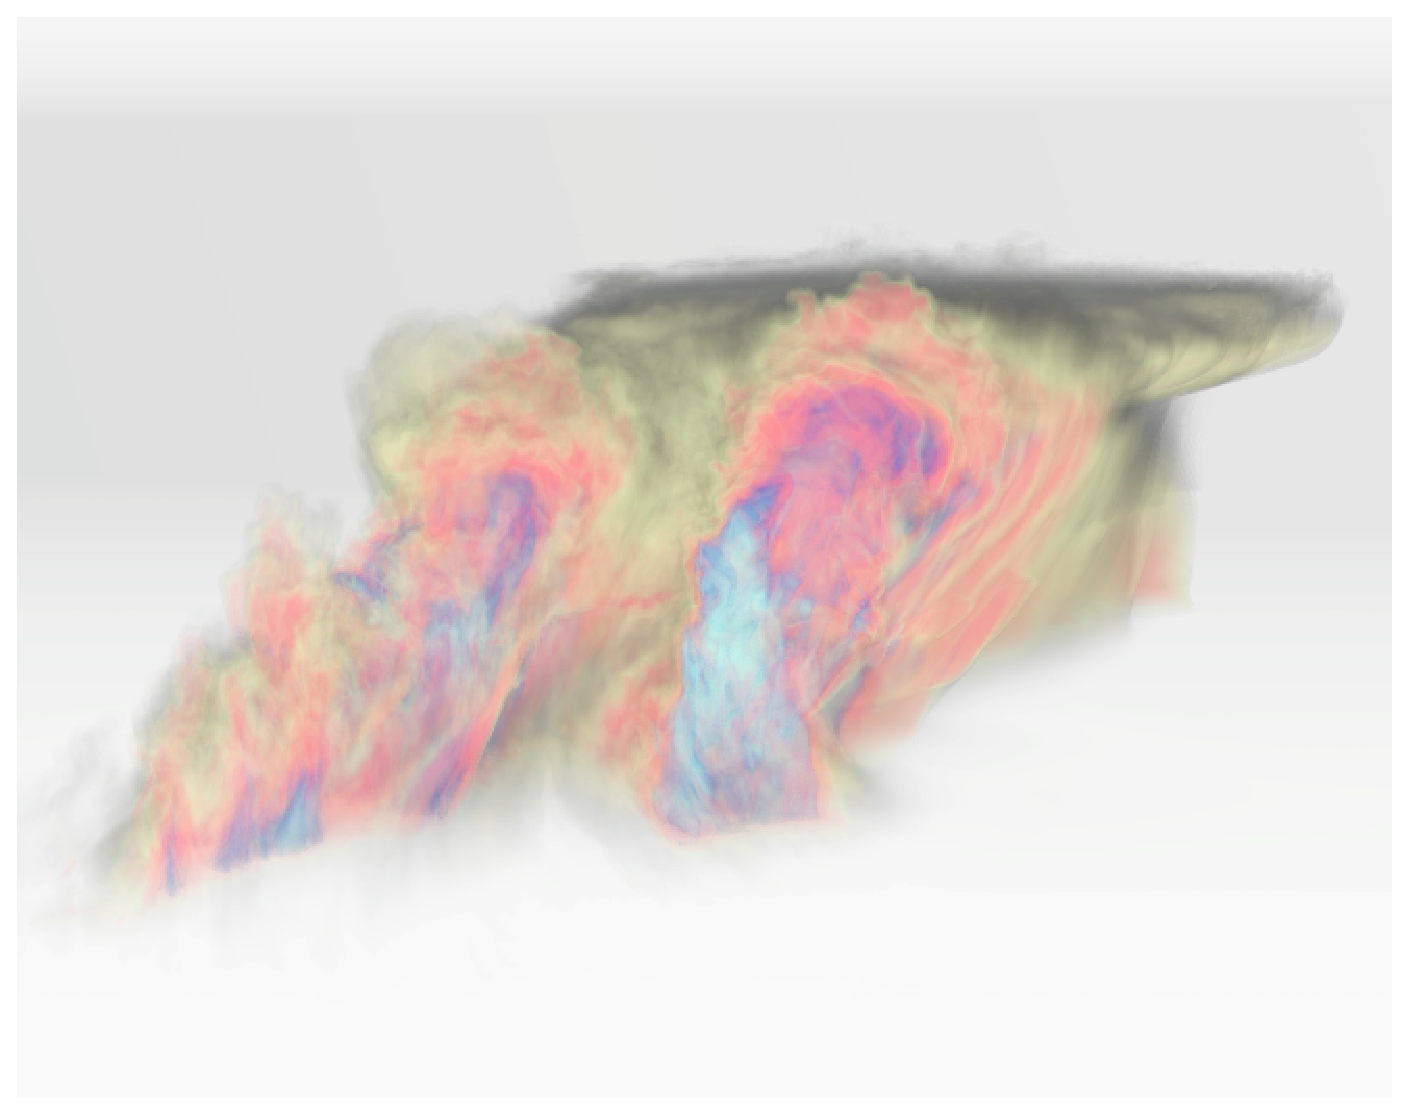
\includegraphics[width=5cm,height=5cm]{figures/cm1-raycasting.eps}}}
	\quad
	\subfigure[CM1 Isosurface]{
	\fbox{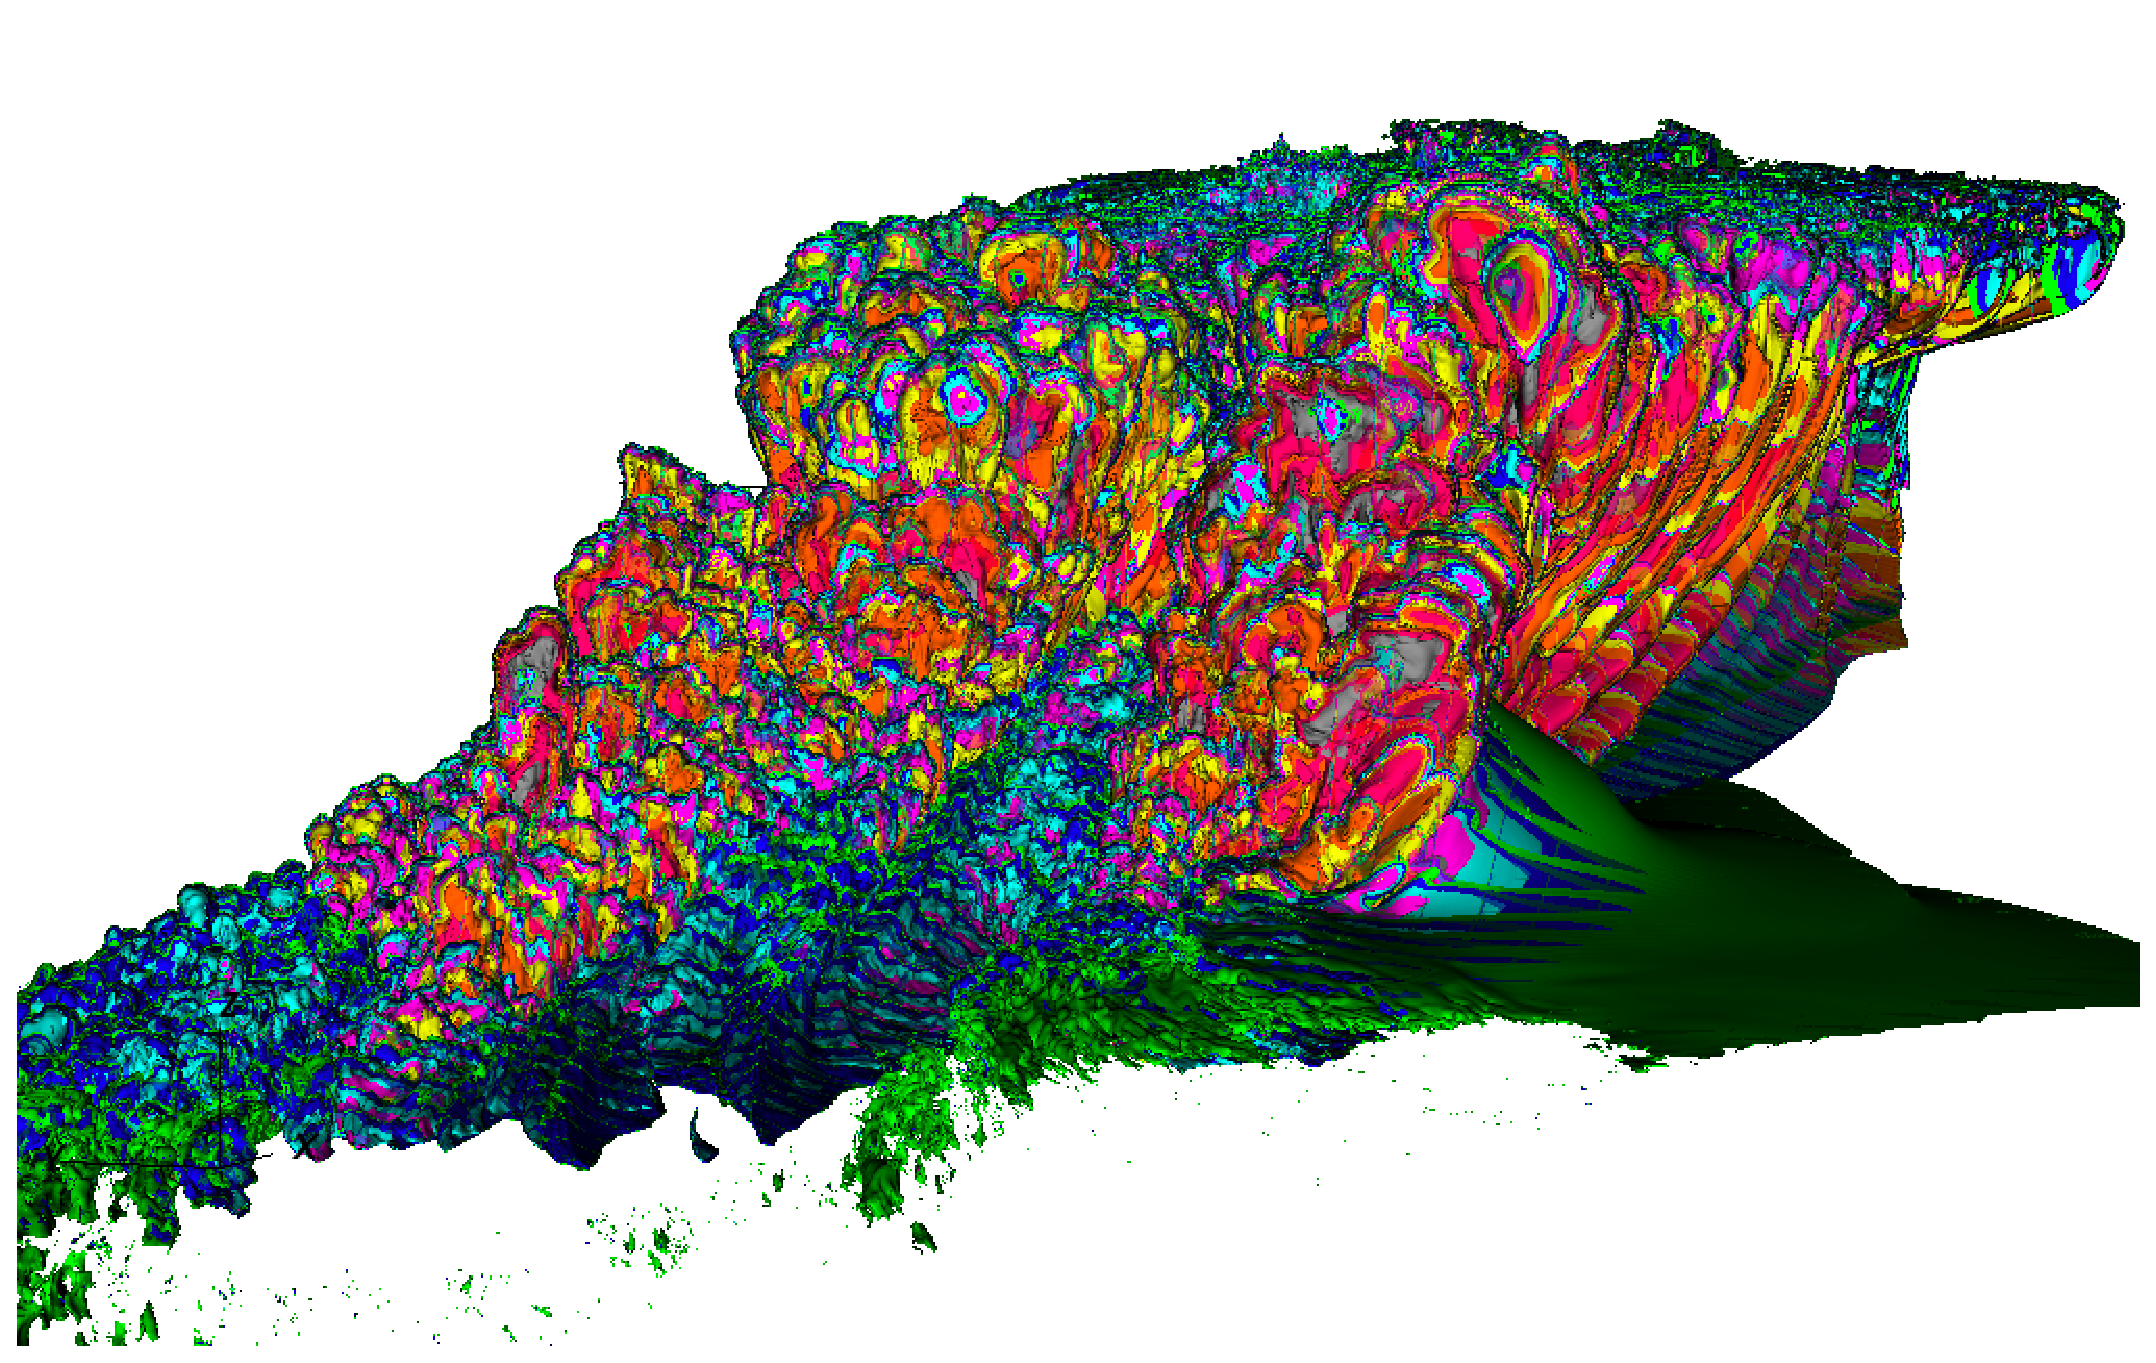
\includegraphics[width=5cm,height=5cm]{figures/cm1-isosurface.eps}}}
	
	\subfigure[CM1 Color Map]{
	\fbox{\includegraphics[width=5cm,height=5cm]{figures/cm1-dbz-colormap.eps}}}
	\quad
	\subfigure[Nek5000 Isosurface]{
	\fbox{\includegraphics[width=5cm,height=5cm]{figures/nek5-volume.eps}}}
	
	\caption[Example of visualizations from the CM1 and Nek5000 simulations]{Example results obtained in situ with Damaris:
	(a) Ray-casting of the \emph{dbz} variable on 6400 cores (Blue Waters).
	(b) 10-level isosurface of the DBZ variable on 6400 cores (Blue Waters).
	(c) Color map of the DBZ variable on 256 cores (Blue Waters).
	(d) Ten-level isosurface of the $y$ velocity field in 
	the TurbChannel configuration of Nek5000.}\label{fig:visualresults}
\end{figure}

The experiments were done on the Blue Waters supercomputer, NCSA's Cray XE6 
Petascale supercomputer~\cite{bluewaters}.
Our goal is to show that ISV approaches depend on the scalability of the rendering algorithm 
being used. We therefore complete a strong-scaling evaluation of two 
rendering methods described bellow.

\paragraph{Methodology}
CM1 requires a long run time before an interesting atmospheric phenomenon appears,
and such a phenomenon may not appear at small scale. Yet, we need visualizable
phenomena to appear in order to evaluate the performance of in situ visualization tasks.
Thus we first ran CM1 with the help of atmospheric
scientists to produce relevant data. We generated a representative dataset of 
$3840 \times 3840 \times 400$ points spanning several iterations.

We then extracted the I/O kernel 
from the CM1 code and built a program that replays its behavior at a given scale 
and with a given resolution by reloading, redistributing and interpolating the 
precomputed data.
The I/O kernel, identical to the I/O part of the simulation, calls Damaris
functions to transfer the data to Damaris. Damaris then performs in situ visualization, 
either in a time-partitioning manner or using dedicated cores.

\paragraph{Time Partitioning vs. Dedicated Cores: Results}
We measured the time to complete a rendering (average of 15 
iterations) using time partitioning and dedicated cores for each scenario. 
The comparative results are reported in Figure~\ref{fig:cm1vistime}.

\begin{figure}[t]
\centering
	\subfigure[In Situ Isosurface]{
	\includegraphics[width=5.5cm]{figures/cm1-in-situ-isosurface.eps}}
	\quad
	\subfigure[In Situ Ray Casting]{
	\includegraphics[width=5.5cm]{figures/cm1-in-situ-ray-casting.eps}}
	\caption[Rendering time of in situ ray-casting and isosurfaces of CM1]{Rendering time using ray-casting and isosurfaces, with 
	time-partitioning and dedicated cores with CM1. Note that the number of cores 
	represents the total number used for the experiments; using a dedicated cores 
	approach, 1/16 of this total number is effectively used for in situ visualization,
	which explains the overall higher rendering time with dedicated cores.}
	\label{fig:cm1vistime}
\end{figure}

The isosurface algorithm scales well with the number of cores 
using both in situ approaches. A time-partitioning approach would thus be 
appropriate if the user does not need to hide the run time impact of in situ 
visualization.
However, on 6400 cores, it takes as much time 
to complete the rendering as on 400 dedicated cores. In
terms of pure computational power, an approach based on dedicated cores is thus 16 
times more efficient.

The ray-casting algorithm on the other hand has a poorer scalability. After 
decreasing, the rendering time goes up again at a 6400-core scale, and it 
becomes about twice more efficient to use a reduced number of dedicated 
cores to complete this same rendering.

\paragraph{Discussion.} The choice of using dedicated cores versus a time-partitioning ISV approach 
depends on (1) the intended visualization scenario, (2) the scale of the experiments and 
(3) the intended frequency of visual output. Our experiments indeed show that at small scale,
the performance of rendering algorithms are good enough to be executed in a time-partitioning manner,
provided that the user is ready to increase the run time of his simulation. At large scale however,
it becomes more efficient to use dedicated cores, especially when using ray-casting,
where the observed rendering performance is substantially better when using a reduced number of
processes.

%%%%%%%%%%%%%%%%%%%%%%%%%%%%%%%%%%%%%%%%%%%%%%%%%%%
% NEK5
%%%%%%%%%%%%%%%%%%%%%%%%%%%%%%%%%%%%%%%%%%%%%%%%%%%

\paragraph{Experiments with the Nek5000 Simulation}
Our goal in this series of experiments is to show the impact of in situ visualization
tasks on the run-time variability of the simulation, and to show how dedicated cores
help alleviating this variability. We show in particular the effect of 
interactivity on this variability. We use the Nek5000 code for this purpose.
In addition to the MATiS configuration already used in Section~\ref{sec:expIO}, we
use the \emph{TurbChannel} configuration, which was designed to run on 32 to 64 cores,
in order to assess the impact of 
interactivity on run time with a time-partitioning approach and with dedicated cores. 
Figure~\ref{fig:visualresults}~(d) shows the result of a 10-level 
isosurface rendering of the fluid velocity along the $y$ axis, with the 
TurbChannel case. We use the MATiS configuration to show the scalability of our 
approach based on Damaris against a standard, time-partitioning approach.

\paragraph{Results with the TurbChannel Configuration}
Experiments were carried out on the Reims \emph{stremi} cluster of the French 
Grid'5000 testbed, which features 40 nodes (HP ProLiant DL165 G7) with 24 cores
per node, connected through a 1G Ethernet network.

To assess the impact of in situ visualization on the run time, we run 
TurbChannel on 48 cores using the two approaches: first we use a 
time-partitioning mode, in which all 48 cores are used by the simulation and 
synchronously perform ISV. Then we switch on one dedicated core per node,
leading to 46 cores being used by the simulation while 2 cores asynchronously run 
the ISV tasks.

In each case, we consider four scenarios: 
\begin{enumerate}
	\item The simulation runs without visualization;
	\item A user connects VisIt to the simulation but does not ask for any output;
	\item The user asks for isosurfaces of the velocity fields but does not interact with VisIt any further 
	(letting the Damaris/Viz update the output after each iteration);
	\item The user has heavy interactions with the simulations (for example rendering different variables, 
using different algorithms, zooming on particular domains, changing the 
resolution).
\end{enumerate}

Figure~\ref{fig:nek5variability} presents a trace of the duration of each
iteration during the four aforementioned scenarios using the two approaches.
Figure~\ref{fig:nek5variability}~(a) shows that ISV using 
a time-partitioning approach has a large impact on the 
simulation run time, even when no interaction is performed. The simple fact of connecting
VisIt without rendering anything forces the simulation to at least update metadata at each iteration,
which takes time.
Figure~\ref{fig:nek5variability}~(b) shows that ISV based on dedicated cores, 
on the other hand, is completely transparent from the point of view of the simulation.

\begin{figure}[t]
\centering
	\subfigure[Time-Partitioning]{
	\includegraphics[width=5.5cm]{figures/turbchannel-time-partitioning.eps}}
	\quad
	\subfigure[Space-Partitioning]{
	\includegraphics[width=5.5cm]{figures/turbchannel-space-partitioning.eps}}
	\caption[Run-time variability in CM1 due to ISV]{Variability 
	in run time induced by different scenarios of in situ 
	interactive visualization.}\label{fig:nek5variability}
\end{figure}

\paragraph{Results with the MATiS Configuration}
We ran the MATiS configuration on 816 cores. Each 
iteration takes approximately one minute and due to the important number of points 
that the mesh contains, it is difficult to perform interactive visualization. 
We therefore connect VisIt and simply query for a 3D pseudo-color plot of the $vx$ 
variable that is then continuously updated.
For the following results, the time-partitioning approach outputs one image every time step,
while dedicated cores adapted the output frequency to one image every 25 
time steps.

Figure~\ref{fig:matisruntime} reports the behavior of the application with and 
without visualization performed, and with and without dedicated cores. 
Corresponding statistics are presented in Table~\ref{tab:matisstats}.

\begin{figure}[t]
\centering
	\subfigure[Time Partitioning, Without Visualization]{
	\includegraphics[width=5.5cm]{figures/matis-tp-no-viz.eps}}
	\quad
	\subfigure[Time Partitioning, With Visualization]{
	\includegraphics[width=5.5cm]{figures/matis-tp-viz.eps}}
	\subfigure[Space Partitioning, Without Visualization]{
	\includegraphics[width=5.5cm]{figures/matis-sp-no-viz.eps}}
	\quad
	\subfigure[Space Partitioning, With Visualization]{
	\includegraphics[width=5.5cm]{figures/matis-sp-viz.eps}}
	\caption[Iteration time of Nek5000's MATiS configuration with and without ISV]{Iteration time 
	of the MATiS configuration without visualization 
	(left) and with visualization enabled (right).
	Top: with time partitioning, visualization time adds to the simulation time. 
	Bottom: With dedicated cores, visualization time entirely overlaps with simulation time.}\label{fig:matisruntime}
\end{figure}

\begin{table}
	\center
\caption[Average iteration time of Nek5000's MATiS configuration]{Average 
	iteration time of the Nek5000 MATiS configuration with a
   time-partitioning approach and with dedicated cores, with and without 
   visualization.}\label{tab:matisstats}
   \begin{tabular}{|l|l|c|c|}
   \hline
\textbf{Iteration Time} & & Average & Std. dev. \\
	\hline
\multirow{2}{*}{Time Partitioning} & w/o vis. & 75.07 sec  & 22,93 \\
	& with vis. & 205.21 sec & 57.15 \\
	\hline
\multirow{2}{*}{Space Partitioning} & w/o vis. & 67.76 sec & 20.09 \\
	& with vis. & 64.79 sec  & 20.44 \\
	\hline
   \end{tabular}
\end{table}

Time-partitioning visualization not only increases the average run time but 
also increases the standard deviation of this run time, making it more unpredictable.
On the other hand, the approach based on dedicated cores yields more consistent results.
One might expect dedicated cores to interfere with the
simulation as it performs intensive communications while the simulation runs. 
However, in practice we observe very little run time variation.

We also remark that decreasing the number of cores used by the simulation actually
decreases its run time. This is due to the fact that Nek5000 reaches its
limit of scalability. Yet due to its memory requirements, it is still necessary to run
it on this number of nodes. In other words, as reducing the number of cores per node
actually used by the simulation increases its performance, it further motivates the
use of these spare cores for extra tasks such as visualization.

Finally, while the  time-partitioning approach performs visualization at every 
time step here, dedicated cores have adapted the frequency of 
its output to 1 image every 25 time steps.
If a time-partitioning approach were to only output 1 image every 25 time steps 
(which corresponds to having only the $25^{th}$ iteration being impacted 
in Figure~\ref{fig:matisruntime} (b)), the completion time for 25 time steps 
would be 2007 seconds on average.
With dedicated cores, this takes 1620 seconds, that is, a 20\% speedup. 
Furthermore, since dedicated cores enable the visualization and 
simulation tasks to overlap, the total run time is unchanged with the addition of ISV.
